\documentclass[twocolumn]{jarticle}
\usepackage{jsaiac}
\usepackage[dvipdfmx]{graphicx}
\usepackage[dvipdfmx]{color}

%%
\title{
\jtitle{人工知能学会テンプレート}
\etitle{jsai report template}
}
%%英文は以下を使用
%\title{Style file for manuscripts of JSAI 20XX}

\jaddress{氏名,所属,住所,電話番号,Fax番号,電子メールアドレスなど}

\author{%
\jname{東大太郎\first}
\ename{Taro TODAI}
\and
\jname{第2筆者氏名\second}
\ename{Second Author's Name}
%\and
%Given-name Surname\third{}%%英文は左を使用
}

\affiliate{
\jname{\first{}人工知能学会}
\ename{The Japanese Society for Artificial Intelligence}
\and
\jname{\second{}所属和文2}
\ename{Affiliation \#2 in English}
%\and
%\third{}Affiliation \#3 in English%%英文は左を使用
}

%%
%\Vol{28}        %% <-- 28th(変更しないでください)
%\session{0A0-00}%% <-- 講演ID(必須)

\begin{abstract}
aaaaaaaaaaaaaaaaaaaaaaaaaaaaaaaaaaaaaaa
aaaaaaaaaaaaaaaaaaaaaaaaaaaaaaaaaaaaaaa
aaaaaaaaaaaaaaaaaaaaaaaaaaaaaaaaaaaaaaa
\end{abstract}

\begin{document}
\maketitle

\section{はじめに}
あああああああああああああああああ
あああああああああああああああああ

\section{関連研究}
あああああああああああああああああ
あああああああああああああああああ
ああああああああああ\cite{imagenet}

\section{提案手法}
あああああああああああああああああ
あああああああああああああああああ\figref{fig:apc} 

\begin{enumerate}
  \item ああああ
  \item いいいい
\end{enumerate} 

\begin{figure}[tbh]
  \centering
  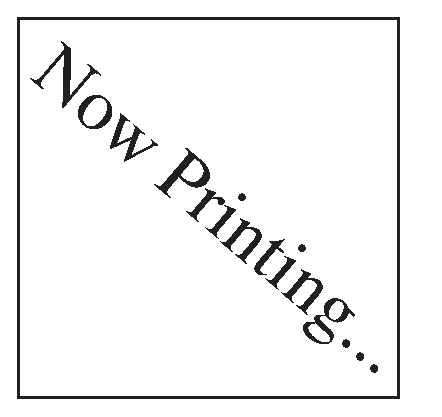
\includegraphics[width=0.7\columnwidth]{figs/nowprinting.eps}
  \caption{TODOTODO}
  \label{fig:apc}
\end{figure}

\section{実験}
あああああああああああああああああ
あああああああああああああああああ

\section{結論}
あああああああああああああああああ
あああああああああああああああああ


\bibliographystyle{jsai}
\bibliography{main}
\end{document}

